\section{Public common-support prediction analysis}\label{sec:s17}
\subsection{Frozen source and observation identity}
The public DrEval files are bound to Zenodo record \nolinkurl{23916090}. The primary sources are \nolinkurl{leaderboard_Nov26.zip} (260,437,238 bytes; MD5 \nolinkurl{1d16cb7ecb59599866c3880e150e81da}) and \nolinkurl{splits.zip} (42,993,448 bytes; MD5 \nolinkurl{e4218bd6c369a4cf8e5235f608ca5ca2}). The separate four-resource source is \nolinkurl{all_results.zip} (2,690,160,813 bytes; MD5 \nolinkurl{e76faf5a2cd41a38007892707e02d8b7}). The accompanying R1 archive retains download hashes, source adapters, frozen aligned predictions and numerical outputs. An offline replay uses those frozen arrays; acquiring and parsing the larger original archives is a separate online reconstruction.

The new target panel selects \texttt{rand\_setting=predictions} and \texttt{test\_mode=LCO}. We first identify keys $(\mathrm{fold},\mathrm{PubChem\ ID},\mathrm{cell\ line})$ occurring once in the official test split. Every accepted predictor record has one matching key, finite prediction and matching truth. The frozen aligned array contains $227{,}510$ source-singleton positions and 34 model columns; finite common intersection gives $106{,}696$ rows for all models and $210{,}741$ for the five-model companion plus its baseline. An official source-row position is retained within each fold. The 106,696-key unique support is exactly the singleton-key subset of the 112,066-row common multiset used in S18; the source-key set and multiplicities are checked directly. These two analyses therefore examine target and measure conditions on nested views of the same fixed public prediction pool. They retain curve-summary identities, without introducing biological replicate identities or reconstructing training.

The five-model companion contains DIPK, ElasticNet, GradientBoosting, RandomForest and SimpleNeuralNetwork, with NaiveMeanEffectsPredictor bound for baseline-normalized reference scores. The broad panel contains 29 non-naive predictors and five naive baselines. Their exact names are retained in the frozen array and the per-model score table, avoiding family-level reinterpretation of a specific configuration.

\subsection{Target definitions and replay}
On the connected LCO reference, unresolved evaluation directions are held-out-cell-line offsets. With $H$ the evaluation cell-membership matrix, $Q=I-H(H^\top H)^+H^\top$. FULL uses the observed $y,p_m$ and ID uses $Qy,Qp_m$. The $R^2$ values are
\[
R^2_{m,\mathrm{FULL}}=1-\frac{\sum_i(y_i-p_{mi})^2}{\sum_i(y_i-\bar y)^2},\qquad
R^2_{m,\mathrm{ID}}=1-\frac{\|Q(y-p_m)\|^2}{\|Qy\|^2}.
\]
Pearson is evaluated on the corresponding raw or projected vectors. The ordinary FULL Pearson in this analysis is different from the baseline-normalized Pearson used in the earlier LDO protocol. We additionally compute the unprojected DrEval normalized score using $y-b,p_m-b$; its common positive $R^2$ denominator preserves within-fold SSE order, but its score levels and fold-average aggregation remain explicitly identified.

The new replay solves sparse membership least-squares systems for $y$ and each stored predictor. Across the broad 340 and companion 60 model--fold records, raw/projected SSE, four $R^2$ variants and three Pearson variants agree with the frozen outputs within the stated tolerances. The maximum absolute scalar discrepancy is $2.9104\times10^{-11}$. No predictive model is fitted by these residualization solves.

For each non-naive model pair, the directed FULL-to-ID sign reversal is counted per fold; persistence requires the same direction in at least seven of ten folds. Median foldwise reversal fractions in the broad panel are $0.0455665$ for $R^2$ and $0.0283251$ for Pearson. Exactly three persistent outcomes occur, all in $R^2$: ElasticNet--MOLIR, KNNRegressor--MOLIR and Lasso--MOLIR, each in ten folds. The five-model companion has medians $0.10$ and $0.05$ with no persistent outcome. These comparisons answer a target-definition question on a verified common support; they do not identify one target as the universally correct scientific task.

The frozen \nolinkurl{RQ3_EFFECT_SIZES_PER_FOLD.csv} retains all thirty A-minus-MOLIR differences. ElasticNet has FULL median/range $0.130452/[0.029012,0.206302]$ and ID $-0.122468/[-0.142156,-0.074123]$; KNNRegressor has $0.127567/[0.033525,0.203026]$ and $-0.094813/[-0.116484,-0.041766]$; Lasso has $0.125710/[0.023039,0.201503]$ and $-0.130655/[-0.155490,-0.081917]$. These are descriptive fold ranges, not confidence intervals. All three pairs share MOLIR and reflect one target distinction.

\subsection{Relationship to the earlier LDO controls}
The earlier seven-model CTRPv2 experiment used registered model-specific post-merge supports and the normalized definitions in Section~S4. Native cross-model occurrence identities were not complete. Its five persistent outcomes therefore remain historical target-sensitivity evidence at that support resolution. The new public LCO panel supplies a separate unique-record comparison; it does not retrospectively replace the old predictions, test split or support contract. Strict GDSC common-support confirmations, the negative GDSC2 persistence result and the one-of-five retraining retention retain their original evidentiary roles.

\begin{table}[htbp]
\centering\small\setstretch{1.08}
\caption{Benchmark ranking changes and cross-fold persistence under \paireval (RQ3). Reversals are directed pair--metric outcomes; the denominator for persistence is ten folds.}
\label{tab:rq3_summary}
\begin{tabularx}{\textwidth}{@{}L{0.22\textwidth}L{0.15\textwidth}L{0.13\textwidth}X@{}}
\toprule
\PAIRTableHead{Cohort and support} & \PAIRTableHead{Median reversal n$R^2$/n$r$} & \PAIRTableHead{Persistent outcomes} & \PAIRTableHead{Ranking and confirmation result}\\\midrule
CTRPv2: 7 models, registered model-specific supports & $0.500/0.357$ & $5$ ($3/2$ by metric) & Archived fixed-prediction realization on registered supports; mean n$R^2$ leader shifts from MultiOmicsNeuralNetwork to DIPK.\\
GDSC2: 6-model common support & $0.30/0.30$ & $0$ & Fold sensitivity exceeds $0.10$, but $0$ persistent pairs ($\ge 7/10$); prespecified two-part primary confirmation is not met.\\
GDSC1: 6-model common support & $0.37/0.33$ & $0$ & Secondary cohort; fold-level sensitivity occurs with $0$ persistent pairs and cannot substitute for GDSC2.\\
Fingerprint-only common support: GDSC2 / GDSC1 & $0.33/0.33$; $0.42/0.33$ & $0$ in both & Secondary support expansion preserves $0$ persistent outcomes in both cohorts.\\
Symmetric-HPO control: 560 jobs & Not summarized here & $1$ of $5$ historical outcomes & Only MultiOmicsNeuralNetwork--RandomForest n$R^2$ retains $\ge 7/10$-fold persistence under new training.\\\bottomrule
\end{tabularx}
\end{table}


\begin{figure}[htbp]
\centering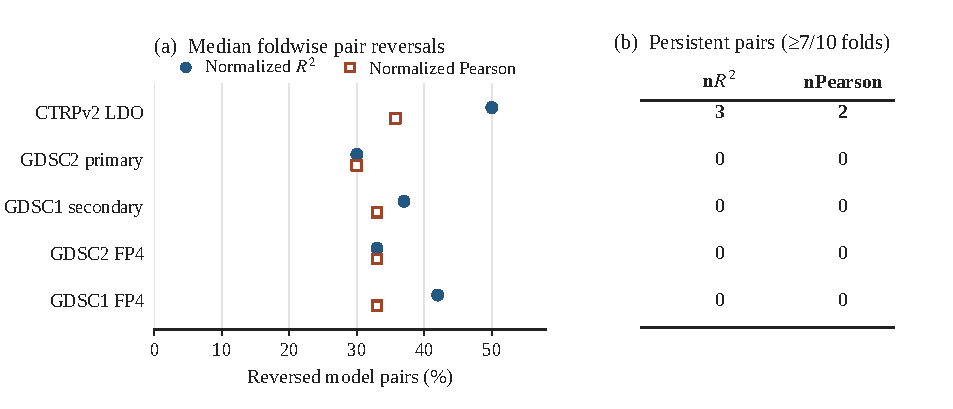
\includegraphics[width=0.96\linewidth]{figures/figure_04.pdf}
\caption{Historical normalized LDO target analysis. \textbf{(a)} Median foldwise reversal fractions by metric. \textbf{(b)} Directed reversals persisting in at least seven of ten folds. The CTRPv2 panel uses registered model-specific supports. Section~S4 describes the GDSC common-support and symmetric-HPO checks.}
\end{figure}

\section{Observation-measure audit and key-repair certificates}\label{sec:s18}
\subsection{Source path, baseline values and support resolution}
The inspected DrEval source is bound to commit \nolinkurl{99c3215dbf9cdac2ba3cbbec2f44ea3bad0d28f6}. The normalization function merges by \texttt{drug\_name}, \texttt{cell\_line\_name} and \texttt{CV\_split}. The checked path does not enforce baseline-key uniqueness and subsequently excludes nonfinite normalized records. Our snapshot reconstruction matches 340 archived primary model--fold normalization entries. Replaying the published function body on three actual model--fold cases additionally agrees with the independent numerical routine to maximum normalized-$R^2$ error $3.06\times10^{-16}$. This function-level adapter is not an installed full-training pipeline.

For the primary common-multiset comparison, source-key counts and truth values must agree for each model, all predictions must be finite, and the repeated target values for each key must be identical. Repeated baseline rows must have one numerical prediction value. We retain each model's original prediction records, and a validated many-to-one identity lookup supplies that value once per record. The primary name and PubChem drug mappings are checked to be bijective. Conflicting baseline values are refused rather than averaged. The common panel has $112{,}066$ original rows per model and $109{,}298$ keys; $2{,}602$ keys have repeated lookup rows. The unchecked join has $117{,}934$ rows per model on this support.

Within repeated keys, no new occurrence ID is invented and no model-to-model pairing of unobserved biological replicate identities is asserted. Identical key truth and multiplicity suffice for the aggregate score/weight comparison. This support resolution is recorded separately from the strict singleton panel in S17 and the native task-row IDs in S20.

\subsection{One-fold SSE and normalized-$R^2$ certificate}
Let $e_{mk}$ be the sum of squared prediction residuals for all original records at key $k$, $d_k=e_{Ak}-e_{Bk}$ and $c_k$ its baseline lookup multiplicity. Then $D=\sum_kd_k$, $D_c=\sum_kc_kd_k$, and correction of $S$ gives
\[
D(S)=D_c-\sum_{k\in S}(c_k-1)d_k.
\]
Sorting the contributions helpful to the unchecked sign gives an upper bound for every fixed-cardinality correction and a feasible first prefix. This proves the minimum strict SSE repair. In one fold, shared positive normalized-$R^2$ denominators reverse the SSE order, so the same minimum applies. The implementation declares a $10^{-12}$ score tolerance and checks the proposed witness directly from sufficient statistics. All 24 foldwise normalized-$R^2$ minima are closed: minimum 1, median 2 and maximum 71 keys.

\subsection{Pearson moments and finite search status}
For a weighted baseline-adjusted target $t_i$ and prediction $q_{mi}$, retain $W=\sum_iw_i$, $S_t=\sum_iw_it_i$, $S_{tt}=\sum_iw_it_i^2$, $S_{q_m}=\sum_iw_iq_{mi}$, $S_{q_mq_m}=\sum_iw_iq_{mi}^2$ and $S_{tq_m}=\sum_iw_it_iq_{mi}$. Define
\[
N_m=WS_{tq_m}-S_tS_{q_m},\qquad K_m=WS_{q_mq_m}-S_{q_m}^2,\qquad
\rho_m=\frac{N_m}{\sqrt{(WS_{tt}-S_t^2)K_m}}.
\]
When both covariance numerators are positive, Pearson order is given by the sign of $N_A^2K_B-N_B^2K_A$. If both are negative its orientation reverses, and mixed signs are handled directly. Key corrections update the raw moments additively, but Pearson is nonlinear in those moments.

The supplied bounds enclose eligible corrected moments and the segment between the original and corrected point. Outward-rounded polynomial interval evaluations bound derivatives and Taylor remainders; bounded search checks candidate leaves directly. A pruning step is applied only when the required covariance signs and variance conditions hold throughout the enclosure. The frozen search closes 34 of 37 minimum counts and retains intervals for the remaining three. Its exact/interval table, selected keys, searched-subset counts, tolerances and logs are preserved. A feasible upper bound or a timed-out search is not relabeled as a minimum.

\begin{table}[htbp]
\centering\small\setstretch{1.02}
\caption{Pearson minimum-key cases retaining certified intervals. These are unresolved minimums with feasible witnesses, not negative search results.}
\begin{tabularx}{\linewidth}{@{}L{0.07\linewidth}XXN{0.10\linewidth}N{0.10\linewidth}@{}}
\toprule
\PAIRTableHead{Fold} & \PAIRTableHead{Model A} & \PAIRTableHead{Model B} & \PAIRTableHead{Lower} & \PAIRTableHead{Upper}\\\midrule
0 & LightGBM & MultiViewNeuralNetwork (gex+mut+fingerp.) & 10 & 12\\
7 & DIPK & XGBoost & 27 & 36\\
7 & DrugGNN & Precily & 16 & 18\\
\bottomrule
\end{tabularx}
\end{table}


\subsection{Averages of foldwise normalized $R^2$}
One-fold SSE sorting does not solve a mean normalized-$R^2$ repair because correcting weights changes the fold denominators. For a current fold with total weight $W$, target mean $\mu$, centered sum of squares $V$ and SSE difference $D$, let a correction remove weight $A$, centered first moment $H$, centered second moment $B$ and SSE difference $U$. Recentring gives
\[
V'=V-B-\frac{H^2}{W-A},\qquad D'=D-U.
\]
Thus a change of $-D/V$ depends on both numerator and denominator. For a fixed cardinality, the implementation bounds removed moments by corresponding largest-contribution sums, requires a strictly positive denominator lower bound, and computes a conservative per-fold improvement bound. A max-plus allocation over folds bounds the improvement of every total-cardinality repair. A verified feasible set of the next cardinality closes the minimum. All five observed mean-$R^2$ minimums are closed, ranging from 5 to 56 with median 8.

The release's portable replay checks all 66 feasible witnesses, re-proves the 24 one-fold SSE cardinalities and the five mean-$R^2$ cardinalities. Pearson search-tree proof receipts are retained; the default replay does not exhaust all those trees again. The R3 audit separately records exhaustive confirmation of 23 Pearson cases whose reported minimum is at most three. These are repeated calculations on the same frozen numerical evidence.

\begin{table}[htbp]
\centering\small\setstretch{1.02}
\caption{Five mean normalized-$R^2$ reversals. Deltas use model A minus model B; larger normalized $R^2$ is preferred. LOFO is the number of ten leave-one-fold deletions retaining the reversal.}
\begin{tabularx}{\linewidth}{@{}L{0.06\linewidth}XN{0.12\linewidth}N{0.12\linewidth}N{0.09\linewidth}N{0.09\linewidth}@{}}
\toprule
\PAIRTableHead{Case} & \PAIRTableHead{A / B} & \PAIRTableHead{Unchecked} & \PAIRTableHead{Repaired} & \PAIRTableHead{Min keys} & \PAIRTableHead{LOFO}\\\midrule
C1 & EnsembleMF / RandomForestAEMolGNet & +0.000765 & -0.001172 & 6 & 3\\
C2 & GradientBoosting / PharmaFormer & -0.001099 & +0.000950 & 5 & 2\\
C3 & GradientBoosting / Precily & +0.006112 & -0.000054 & 40 & 3\\
C4 & MultiViewXGBoost (gex+mut+fingerp.) / XGBoost & -0.000801 & +0.000465 & 8 & 1\\
C5 & PharmaFormer / Precily & +0.007211 & -0.001004 & 56 & 4\\
\bottomrule
\end{tabularx}
\end{table}


All $2{,}602$ duplicate keys lie in 15 cell-line lookup groups and involve 337 drug IDs. Treating an entire cell-line lookup group as a correction action gives a different intervention: minimum 1--2 groups for foldwise cases and 1--4 for mean cases. Exhaustive subset checks over the observed groups certify those counts. Neither a key nor a group count is an annotation budget, a new experimental sample count or a statistical significance statement.

\subsection{Decision materiality and coverage controls}
The $61$ fold pair--metric reversals comprise $24/4{,}060$ normalized-$R^2$ and $37/4{,}060$ Pearson outcomes. Mean comparisons contain five normalized-$R^2$ and zero Pearson reversals. Neither mean-score first place changes; EnsembleMF and RandomForestAEMolGNet exchange third and fourth place under mean normalized $R^2$. The original R3 table columns \texttt{expanded\_rank\_*} contain the repaired once-weighted ranks despite their inherited names. The integrated figures and knowledge records use the numerical values and explicit unchecked/repaired labels.

Four mean reversals have no fold-level sign reversal for that pair. Changes in each fold's advantage alter the average preference. Leave-one-fold-out reaggregation retains the five mean reversals in 3, 2, 3, 1 and 4 deletions, respectively, in the table's order. No case has absolute before/after margins of at least $0.005$ on both sides. These descriptive checks distinguish a real numerical change from a large or stable model-selection consequence.

Baseline-coverage checks apply the current fixed filter to four external resources. The five-model primary common panels have no pair reversals on GDSC2, GDSC1, CCLE or CTRPv1. Their covered/removed row counts and secondary panels are in the supplied coverage tables. The secondary eight-model GDSC2 panel loses $3{,}735$ of $132{,}951$ common rows and has one fold normalized-$R^2$ change; its mean leader is unchanged. The exact current-source function body reproduces this witness. Historical normalized archive values on some external resources do not have a fully reconstructed production contract, so this diagnostic is not an assertion about those historical values or the formal DrEval article.

\section{Missing-score and task-population decision bounds}\label{sec:s19}
\subsection{AMLB frozen cleaning and observed absent job}
The results repository is bound to \nolinkurl{43a87ff4c44f847f5c785ca1c8714c8e9ddfb7f0}; the associated benchmark reporting code is bound to \nolinkurl{dfe8d21871e2dec2b7cab6c9fbfe3575ce4dadc6}. The original data files, cleaning notebook, processing functions and reporting source carry file hashes and Git-blob identities. Reconstructing the frozen rules reproduces 29,829 score entries. Explicit failed jobs use the registered constant-predictor fallback, and a documented special fallback retains its source rule. An actually absent row is kept distinct from a present failed job.

For \texttt{socmob} (OpenML task 359932), \texttt{autosklearn}, constraint \texttt{4h8c\_gp3}, fold 9 is absent. The nine observed $-\mathrm{RMSE}$ values sum to $S=-109.38623$. Let $x\le0$ denote the unknown tenth value. Its completed ten-fold task mean is $(S+x)/10$. For each fixed competing task mean $b_j$, a rank crossing can occur only at $x=10b_j-S$. Negative crossings, their tie points, the endpoint $0$ and one representative of every intervening/tail interval therefore cover the entire domain. The regression panel evaluates 26 boundary/interval states and the all-task panel 22; these are enumeration states and need not be different final ranking vectors.

Across these states, AutoGluon(B) is the unique global winner of both panels. The regression top three are AutoGluon(B), H2OAutoML and flaml; the all-task top three are AutoGluon(B), H2OAutoML and lightautoml. Minimum global mean-rank winner gaps over the domain are 1.181818 and 1.586538, respectively. The constant-baseline value $-43.8865$ is separately evaluated as a declared fallback scenario, not recovered missing truth. No finite lower bound on the unknown true score is assumed. These conclusions fix the other scores, available frameworks and mean-rank policy, and concern the analysis snapshot rather than an attributed error in the JMLR article.

\subsection{Conditional deletion of complete observed tasks}
For rank matrix $r_{mt}$, the comparison between original winner $A$ and challenger $B$ after task deletions depends on $D(S)=\sum_t(r_{Bt}-r_{At})-\sum_{t\in S}(r_{Bt}-r_{At})$. The denominator $|T\setminus S|$ is positive for every allowed set. Therefore strict reversal occurs exactly when $D(S)<0$. Descending prefixes of task contributions bound every possible deletion set of the same size. Ties use a non-strict threshold and are reported separately. Doubled ranks are checked as integers, avoiding tolerance-based tie decisions.

\begin{table}[htbp]
\centering\small\setstretch{1.02}
\caption{Frozen mean-rank panels: minimum task deletions for loss of a strict winner (tie allowed) and for a strict challenger improvement. Single-task top-three ties are recorded separately.}
\begin{tabularx}{\linewidth}{@{}L{0.08\linewidth}XN{0.08\linewidth}N{0.11\linewidth}N{0.10\linewidth}N{0.14\linewidth}N{0.13\linewidth}@{}}
\toprule
\PAIRTableHead{Budget} & \PAIRTableHead{Panel} & \PAIRTableHead{Tasks} & \PAIRTableHead{Tie/loss} & \PAIRTableHead{Strict} & \PAIRTableHead{Top-3 changes} & \PAIRTableHead{Top-3 ties}\\\midrule
1h & Regression & 33 & 10 & 11 & 9 & 1\\
1h & AUC & 41 & 14 & 14 & 4 & 0\\
1h & Negative log loss & 30 & 20 & 20 & 0 & 0\\
1h & All tasks & 104 & 38 & 39 & 0 & 0\\
4h & Regression & 33 & 6 & 6 & 0 & 0\\
4h & AUC & 41 & 6 & 7 & 0 & 0\\
4h & Negative log loss & 30 & 11 & 11 & 0 & 0\\
4h & All tasks & 104 & 29 & 29 & 0 & 0\\
\bottomrule
\end{tabularx}
\end{table}


All 94 challenger comparisons retain either a minimum with a concrete deletion set and a previous-cardinality lower bound, or a proof that no nonempty remainder permits a strict overturn. The integrated alternate checker reuses the original data cleaning and panel builder, while checking the integer prefix and witness predicates without calling its optimization routine. The original driver is also rerun. Random small-panel exhaustive checks generate 250 panels, exclude 29 with tied initial leaders, and verify all nonempty proper deletion subsets on the remaining 221. These checks establish the implementation's finite behavior and do not add independent benchmark observations.

The task intervention changes the evaluation population. A small conditional deletion threshold does not establish missing tasks in the source, nor does a large threshold establish general algorithmic superiority. For the actual absent fold and the counterfactual task deletions, the certificate records different domains and different meanings.

\section{Canonical prediction identity and numerical production scope}\label{sec:s20}
\subsection{TabArena native common defaults}
The Mitra\_GPU cache is the complete \nolinkurl{tabarena-2025-09-03/methods/Mitra_GPU/raw.zip}, SHA256 \nolinkurl{c0150562740472ee73d8b7a6bc48690ce37b33d71bdc108b4a649f1f314d0dcb}. It contains 654 default-configuration records over 33 tasks. The LightGBM source is \nolinkurl{tabarena-2025-06-12/methods/LightGBM/raw.zip}; only the 654 matching original members are retrieved with conditional range requests, original CRC checks and retained member SHA values. The full 44.99-GB LightGBM archive is not redistributed or given a claimed whole-file hash. The source ETag, byte ranges and selected-member provenance are retained.

Each model has 17 tasks with 30 evaluation units and 16 tasks with nine units. The native task metadata identifies task, repeat, fold, sample and row IDs. Directory order is \texttt{repeat\_fold}; \texttt{split\_idx} is stored separately and is mapped to flattened score-table fold by the pinned source. We compare the score carried by each native record rather than claiming to reconstruct the entire public leaderboard. The common panel is determined by native default availability, with no outcome-based task selection.

Canonical task descriptions, split ARFF files, exact dataset-version metadata and target columns are acquired for all 33 tasks. Dataset row position is the source row ID. Native test membership, order, decoded class labels and regression targets agree with those sources in all 1,308 model records. Native validation labels also match and their identities belong to the declared train partition. Test identities are unique and disjoint from validation identities. Repeated splits and the two model copies are not independent samples.

\begingroup\small\setstretch{1.0}
\begin{longtable}{@{}L{0.13\linewidth}L{0.43\linewidth}L{0.16\linewidth}N{0.16\linewidth}@{}}
\caption{Canonical TabArena task coverage. Units are common task-repeat-fold-sample records per model; all corresponding test identity, order and truth checks pass.}\\
\toprule \PAIRTableHead{Task ID} & \PAIRTableHead{Dataset} & \PAIRTableHead{Metric} & \PAIRTableHead{Units/model}\\\midrule\endfirsthead
\toprule \PAIRTableHead{Task ID} & \PAIRTableHead{Dataset} & \PAIRTableHead{Metric} & \PAIRTableHead{Units/model}\\\midrule\endhead
363612 & airfoil\_self\_noise & rmse & 30\\
363614 & anneal & log\_loss & 30\\
363615 & Another-Dataset-on-used-Fiat-500 & rmse & 30\\
363619 & Bank\_Customer\_Churn & roc\_auc & 9\\
363621 & blood-transfusion-service-center & roc\_auc & 30\\
363623 & churn & roc\_auc & 9\\
363624 & coil2000\_insurance\_policies & roc\_auc & 9\\
363625 & concrete\_compressive\_strength & rmse & 30\\
363626 & credit-g & roc\_auc & 30\\
363629 & diabetes & roc\_auc & 30\\
363632 & E-CommereShippingData & roc\_auc & 9\\
363671 & Fitness\_Club & roc\_auc & 30\\
363674 & hazelnut-spread-contaminant-detection & roc\_auc & 30\\
363675 & healthcare\_insurance\_expenses & rmse & 30\\
363676 & heloc & roc\_auc & 9\\
363681 & in\_vehicle\_coupon\_recommendation & roc\_auc & 9\\
363682 & Is-this-a-good-customer & roc\_auc & 30\\
363684 & Marketing\_Campaign & roc\_auc & 30\\
363685 & maternal\_health\_risk & log\_loss & 30\\
363686 & miami\_housing & rmse & 9\\
363689 & NATICUSdroid & roc\_auc & 9\\
363691 & online\_shoppers\_intention & roc\_auc & 9\\
363694 & polish\_companies\_bankruptcy & roc\_auc & 9\\
363696 & qsar-biodeg & roc\_auc & 30\\
363698 & QSAR\_fish\_toxicity & rmse & 30\\
363700 & seismic-bumps & roc\_auc & 9\\
363702 & splice & log\_loss & 9\\
363704 & students\_dropout\_and\_academic\_success & log\_loss & 9\\
363706 & taiwanese\_bankruptcy\_prediction & roc\_auc & 9\\
363707 & website\_phishing & log\_loss & 30\\
363708 & wine\_quality & rmse & 9\\
363711 & MIC & log\_loss & 30\\
363712 & jm1 & roc\_auc & 9\\
\bottomrule\end{longtable}
\endgroup


\subsection{Metric definitions and alternate numerical replay}
The panel has 348 binary 1-AUC, 138 multiclass log-loss and 168 regression RMSE records per model. RMSE is computed after converting predictions to Float64. AUC uses average-rank tie handling. For log loss, probabilities are converted to Float64 and row-normalized; the correct-class probability is clipped to $[10^{-15},1]$ and the negative log is averaged. A second arithmetic implementation uses \texttt{math.fsum}, Mann--Whitney ranks and direct normalized log probabilities, agreeing on all 1,308 point metrics with maximum scaled discrepancy $3.43\times10^{-16}$.

The current source is fixed at \nolinkurl{bfa8c50c17885e5b722d75ce5bcb5db3822257a3}. Its \nolinkurl{AGBagResult._pred_test_from_children} function body is executed directly on the stored child forecasts. All 1,308 aggregated predictions equal the stored test forecasts. For legacy records lacking per-child validation predictions, only the shape consulted by the test aggregator is supplied from the corresponding test-child shape; validation-child alignment is not claimed to be replayed. The complete historical model training/inference/scoring pipeline is not identified by this current-source calculation.

\paragraph{Observed margin relative to score deviations.}
For unit $u$, write $e_{m,u}^{\rm native}$ and $e_{m,u}^{\rm cache}$ for the stored and reconstructed model errors, and put $b_u=|e_{A,u}^{\rm cache}-e_{A,u}^{\rm native}|+|e_{B,u}^{\rm cache}-e_{B,u}^{\rm native}|$. The triangle inequality bounds the difference between the two observed pair gaps by $b_u$. Over units with $b_u>0$, the minimum $|e_{A,u}^{\rm cache}-e_{B,u}^{\rm cache}|/b_u$ is $32.0$. This descriptive ratio uses the observed native/cache differences and is distinct from an a priori enclosure of unknown historical internal predictions.

\subsection{Conditional Float32 cells and unresolved origin}
For cached Float32 prediction $p_i$, let $p_i^-$ and $p_i^+$ be the midpoints to its adjacent floating values. The diagnostic assumes the unknown internal prediction lies in this cell through one storage rounding. RMSE bounds use the nearest and farthest residual in each cell. AUC uncertainty is bounded by positive--negative pairs tied at the same cached score; strictly ordered Float32 values preserve their order under this model. Log-loss bounds enclose the normalized correct-class probability before the declared clipping. These are deterministic conditional enclosures, with 450 constructed numerical checks.

Native-to-cache maximum absolute differences are $0.00206269$ for RMSE, $5.7671\times10^{-5}$ for 1-AUC and $9.8935\times10^{-9}$ for log loss. RMSE's maximum relative difference is approximately $4.62\times10^{-7}$. Of 1,308 native fields, 1,265 are compatible with the one-rounding model, while 43 are outside it: 37 log-loss fields on \texttt{anneal} and six AUC fields across \texttt{churn}, \texttt{credit-g}, \texttt{in\_vehicle\_coupon\_recommendation}, \texttt{qsar-biodeg} and \texttt{E-CommereShippingData}. The 43 fields concern 31 evaluation units and six tasks. Compatibility does not identify a producer, and incompatibility does not establish a benchmark bug when historical internal predictions and arithmetic are absent.

Four conditional pair intervals straddle zero, all on \texttt{blood-transfusion-service-center}; the observed native-to-cache signs are unchanged. All 33 task-average intervals have a strict direction under the stated cell model. The unknown historical producer is kept unresolved even for a conditionally strict interval. A separate regrouping check on the derived CSV fields finds that every observed cache score gap exceeds the sum of the two observed native-to-cache deviations, with minimum ratio $32.0$. This is a post-hoc description of those two score versions, not a bound over arbitrary unseen historical or future production paths.

\section{Comparison-object implementation and integrated reproduction}\label{sec:s21}
\subsection{Portable records and graph links}
The evaluation slice of the integrated adapter exports 872 selected comparison assertions with linked contract, model and evidence nodes. The assertions comprise three persistent target switches, 66 lookup-repair outcomes, 22 actual missing-score winner comparisons, 94 task-deletion certificates and 687 TabArena unit/task-mean comparisons. These counts describe software materializations from the evidence already analyzed, not new observations or independent discoveries.

A record has a schema version, study, claim kind, models, comparison contract, outcome, witness and evidence bindings. The contract includes target and measure semantics, metric orientation, aggregation, intervention domain/unit and input-snapshot digests. A canonical-content digest identifies the record and its contract. Source archive/member digests bind the retained numerical evidence. Concrete repair keys and task-deletion witnesses are retained in the records. Typed predicates validate a strict repair sign change, a minimum-cardinality witness, a preference interval or a persistence threshold. For a local molecular relation, the numerical checker verifies generalized-inverse binding and the four reference/source/readout identities. Hash validation and numerical validity remain different operations.

The JSON-LD graph represents models, comparison assertions, contracts and evidence entities, with PROV derivation links. The namespace is a local \texttt{urn:pair:} vocabulary; no external ontology registration or graph reasoning service is assumed. Numerical payloads and witness fields remain available in the companion JSON Lines file. Four implemented record queries return changed mean-repair preferences, actual missing-score winner certificates, conditional numerical boundaries, and task-deletion certificates; a summary query counts each category. Three SPARQL queries return five, 22 and four records for the first three categories, respectively, on the parsed JSON-LD graph. A producer-unresolved field remains queryable in all relevant TabArena records.


\paragraph{Actual missing-fold certificates.}
The final adapter adds $22$ winner--challenger records derived from the two R4 panels, with $13$ and $11$ frameworks. Each binds the unknown $x=-\mathrm{RMSE}\le0$, the nine observed scores, framework set and mean-rank rule. The witness contains analytic mean-rank endpoints and a positive conservative pair gap. The independent endpoint checker verifies all $48$ reported mean-rank interval endpoints. The top-three certificate compares the largest upper endpoint among the three members with the smallest lower endpoint outside that set. The exported bounds are conservative paired enclosures; the regime enumeration remains the more precise joint-domain calculation. These records represent the existing two-panel missing-score result.

\paragraph{Coverage of the research line.}
The supplied result-to-manuscript map links the original scientific audit, the synthetic contract verifier, the public prediction audit and R2--R6 numerical results to the formal statements, main results, supplementary details and executable evidence. The original early synthetic scripts are retained and rerun; their checks contribute no empirical observations. Two repaired R4 wrappers have identical bytes for $64$ shared scientific payload members; their differences are packaging metadata and the repair note. Both are retained, with the identity comparison, so they cannot be mistaken for independent experiments. The alternative November-16 KBS writing branch is also frozen for editorial comparison.

\subsection{Commands and actual execution coverage}
The supplied package contains every dated public-evidence bundle used by the integrated driver, including their nested manifests and third-party notices. From the manuscript source directory, run
\begin{quote}\small\ttfamily
bash RUN\_PUBLIC\_EVIDENCE.sh /absolute/new\_output\_directory
\end{quote}
after installing the declared Python dependencies. The output directory must be new. The driver verifies input archive hashes and CRCs, checks that embedded R3/R5 files match the separately supplied versions, and runs sequential stages: the original scientific geometry and synthetic contract checks, exact rational reference/measure fixtures, R1 frozen-prediction/witness replay, full public target-score replay, R2 repair witnesses/minimum bounds, R2 coverage witness, R4 AMLB plus R3 replay, R6 native prediction/reference plus nested R5 replay, object compilation, constructed semantic checks and exported-record verification, followed by RDF parsing and SPARQL query checks. The actual integrated execution receipt records the exit code of every stage.

The R4 archive used here includes the restored nested R3 \texttt{SHA256SUMS.json}; it is byte-identical to the file in its embedded original R3 archive. The old omission affected offline packaging, and the repair changes no scientific input or conclusion. The final reproduction package retains nested checksum manifests rather than excluding every file with a checksum basename. Manuscript/figure compilation and final-archive fresh-directory execution have separate receipts.

The R1 target reconstruction, R2 sufficient-statistic checks, R4 job-score replay and R6 raw cached-prediction replay have different evidence resolutions. None retrains the predictive models. The 340 primary normalization values and historical Pearson-search proofs retain their original source-reconstruction/search receipts; the default offline driver does not reacquire all multi-gigabyte public archives or rerun every Pearson branch tree. The original fetch/reconstruction programs are preserved for that purpose.

\subsection{Relation to historical materials in S6 and S15}
Sections S6 and S15 describe the earlier APA/LDO author-side archive and its bounded public scorer snapshot. Their missing original producer inputs are not supplied by the new public prediction panels. Conversely, the frozen inputs for the new S17--S20 numerical analyses are included in this reproduction distribution. Their identities and scopes are recorded separately, so an old missing-input statement is not incorrectly extended to the new panels and a new public-data replay is not used to certify an absent historical producer.

The executable analyses use the same frozen inputs and a recorded computational environment. Alternate formulas provide numerical cross-checks on those data and do not add an external replication. Molecular structural dimensions, descriptive covariance, observed evaluation changes and counterfactual robustness bounds preserve their own statistical units. This separation is part of the contract exported with each result.

Section~S22 extends this evaluation slice with 24 actual conditional molecular version objects and a matched classical composition.
